\section{Import \& Export}

\subsection{Import}

\begin{figure}
  \centering
  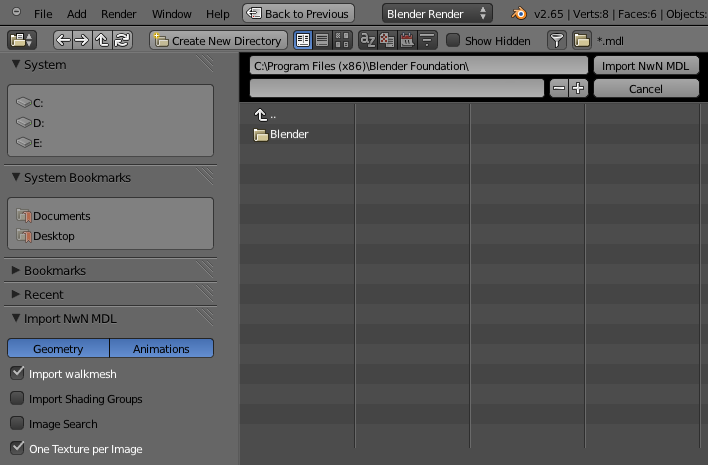
\includegraphics[trim=0 0 0 0, clip, width=\textwidth]{import01}
  \caption[mdl import]{Import Screen}
  \label{fig:import01}
\end{figure}

\begin{description}
    \item[Import Geometry] Import the geometry from the mdl file
    \item[Import Walkmesh] Attempts to import a walkmesh. If the imported model is a placeable, the script will look for a {\textit{*.pwk}} file in the same folder. If the model is a door, it will look for a {\textit{*.dwk}} file. If the model is a tile, it will read the walkmesh directly from the {\textit{*.mdl}} file.
    \item[Import Smooth Groups] Import smooth groups as sharp edges.
    \item[Import Animations] Import animation from the mdl file. Animations are added to the imported geometry. If no geometry has benn imported, the script will try to add animations the already existing objects in blender.
    \item[Materials] None = No materials or textures will be imported. Single = The script will attempt to merge similar materials to reduce clutter. Multiple = Each object will get it's own material, even if this results in multiple identical materials.
    \item[Image Search] Search for textures in subdirectories. This might take a significant amount of time depending on the number of files.
\end{description}


\subsection{Export}

\subsubsection*{Export Options}
\begin{description}
    \item[Export Animations] ported regardless of this setting.
    \item[Export Walkmesh] Attempts to export a walkmesh. The type of exported walkmeshes depends on the objects classification.
    \item[Export Smooth Groups] Convert sharp edges to smooth groups.
    \item[Apply Modifiers] Apply Modifiers before exporting.
\end{description}
